\documentclass[12pt,a4paper]{article}

% ─── Page Layout ───────────────────────────────────────────────────────────────
\usepackage[a4paper, margin=0.8in, headheight=14pt]{geometry}

% ─── Fonts (XeLaTeX) ───────────────────────────────────────────────────────────
\usepackage{fontspec}
\usepackage{unicode-math}
\setmainfont{TeX Gyre Pagella}
\setmonofont[Scale=0.88]{TeX Gyre Cursor}
\setmathfont{Latin Modern Math}

% ─── Packages ──────────────────────────────────────────────────────────────────
\usepackage{xcolor}
\usepackage{colortbl}
\usepackage{titlesec}
\usepackage{enumitem}
\usepackage{tabularx}
\usepackage{booktabs}
\usepackage{array}
\usepackage{amsmath}
\usepackage{tikz}
\usetikzlibrary{shapes.geometric, arrows.meta, positioning, calc, fit, decorations.pathreplacing}
\usepackage{tcolorbox}
\tcbuselibrary{skins, breakable}
\usepackage{hyperref}
\usepackage{fancyhdr}
\usepackage{graphicx}
\usepackage{microtype}
\hyphenpenalty=10000
\exhyphenpenalty=10000
\sloppy
\usepackage{caption}
\usepackage{setspace}
\usepackage{multirow}
\usepackage{tocloft}

% ─── Q&A helper ────────────────────────────────────────────────────────────────
\newcommand{\Q}[1]{\textbf{#1}\par\noindent\ignorespaces}

% ─── Colour Palette ────────────────────────────────────────────────────────────
\definecolor{myred}{RGB}{196,30,58}
\definecolor{mydark}{RGB}{30,30,50}
\definecolor{mygreen}{RGB}{14,120,80}
\definecolor{myteal}{RGB}{0,130,140}
\definecolor{myamber}{RGB}{180,100,0}
\definecolor{mypurple}{RGB}{100,30,160}
\definecolor{mygray}{RGB}{246,247,249}
\definecolor{mgframe}{RGB}{180,185,200}
\definecolor{watermark}{RGB}{145,150,170}
\definecolor{hdrred}{RGB}{250,232,235}
\definecolor{hdrgreen}{RGB}{220,244,233}
\definecolor{hdrteal}{RGB}{220,242,244}
\definecolor{hdramber}{RGB}{253,242,215}
\definecolor{hdrpurple}{RGB}{238,228,255}
\definecolor{hdrgray}{RGB}{238,240,245}
\definecolor{rowalt}{RGB}{250,251,253}

% ─── Section Formatting ────────────────────────────────────────────────────────
\titleformat{\section}
  {\large\bfseries\color{myred}}{\thesection.}{0.5em}{}
  [\vspace{1pt}{\color{myred}\rule{\linewidth}{0.8pt}}]
\titleformat{\subsection}
  {\normalsize\bfseries\color{myteal}}{\thesubsection}{0.5em}{}
\titlespacing*{\section}{0pt}{18pt}{7pt}
\titlespacing*{\subsection}{0pt}{11pt}{4pt}

% ─── Paragraph ─────────────────────────────────────────────────────────────────
\setlength{\parindent}{0pt}
\setlength{\parskip}{4pt}

% ─── TOC Styling ───────────────────────────────────────────────────────────────
\renewcommand{\cfttoctitlefont}{\large\bfseries\color{myred}}
\renewcommand{\cftaftertoctitle}{\par\noindent{\color{myred}\rule{\linewidth}{0.8pt}}}
\setlength{\cftbeforetoctitleskip}{0pt}
\setlength{\cftaftertoctitleskip}{6pt}
\renewcommand{\cftsecfont}{\normalsize\bfseries\color{mydark}}
\renewcommand{\cftsecpagefont}{\normalsize\bfseries\color{mydark}}
\renewcommand{\cftsecleader}{\cftdotfill{\cftdotsep}}
\setlength{\cftbeforesecskip}{7pt}
\renewcommand{\cftsubsecfont}{\small\color{mydark}}
\renewcommand{\cftsubsecpagefont}{\small\color{mydark}}
\setlength{\cftbeforesubsecskip}{3pt}
\setlength{\cftsubsecindent}{1.4em}

% ─── Table helpers ─────────────────────────────────────────────────────────────
\renewcommand{\arraystretch}{1.45}
\setlength{\tabcolsep}{6pt}
\arrayrulecolor{mydark}
\newcolumntype{B}[1]{>{\small\bfseries\raggedright\arraybackslash}m{#1}}
\newcolumntype{Y}{>{\small\raggedright\arraybackslash}X}
\renewcommand{\tabularxcolumn}[1]{m{#1}}

% ─── Header / Footer ───────────────────────────────────────────────────────────
\pagestyle{fancy}
\fancyhf{}
\fancyhead[L]{\small\color{myred}\textbf{PE-EC603C}\;\color{mydark}--- CMOS VLSI Design}
\fancyhead[R]{\small\color{myteal}\textbf{Module 6 Notes}}
\fancyfoot[C]{\small\color{mydark}\thepage}
\fancyfoot[R]{\small\color{watermark}\textit{\copyright\ Biraj Sarkar}}
\renewcommand{\headrulewidth}{0.5pt}
\renewcommand{\footrulewidth}{0.3pt}

% ─── Hyperref ──────────────────────────────────────────────────────────────────
\hypersetup{
  colorlinks=true, linkcolor=myteal, urlcolor=myteal,
  pdfauthor={Biraj Sarkar},
  pdftitle={PE-EC603C --- Module 6 Notes}
}

% ─── tcolorbox styles ──────────────────────────────────────────────────────────
\tcbset{
  tikzbox/.style={
    colback=mygray, colframe=mgframe, boxrule=0.6pt, arc=4pt,
    left=8pt, right=8pt, top=6pt, bottom=6pt,
    colbacktitle=mgframe, coltitle=mydark,
    fonttitle=\small\bfseries
  },
  defbox/.style={
    colback=hdrgreen, colframe=mygreen, boxrule=0.8pt, arc=4pt,
    left=9pt, right=9pt, top=6pt, bottom=6pt,
    colbacktitle=mygreen, coltitle=white,
    fonttitle=\small\bfseries
  },
  formulabox/.style={
    colback=hdrteal, colframe=myteal, boxrule=0.8pt, arc=4pt,
    left=9pt, right=9pt, top=7pt, bottom=7pt,
    colbacktitle=myteal, coltitle=white,
    fonttitle=\small\bfseries
  },
  examplebox/.style={
    colback=hdramber, colframe=myamber, boxrule=0.8pt, arc=4pt,
    left=9pt, right=9pt, top=6pt, bottom=6pt,
    colbacktitle=myamber, coltitle=white,
    fonttitle=\small\bfseries
  },
  masonbox/.style={
    colback=hdrpurple, colframe=mypurple, boxrule=0.8pt, arc=4pt,
    left=9pt, right=9pt, top=6pt, bottom=6pt,
    colbacktitle=mypurple, coltitle=white,
    fonttitle=\small\bfseries
  },
  exambox/.style={
    colback=hdrpurple, colframe=mypurple, boxrule=1pt, arc=5pt,
    left=10pt, right=10pt, top=8pt, bottom=8pt,
    colbacktitle=mypurple, coltitle=white,
    fonttitle=\bfseries,
    breakable, title after break={\textbf{Frequently Asked / Viva Questions (contd.)}}}
}
% Make all boxes breakable across pages
\tcbset{breakable}

% ─── TikZ styles ───────────────────────────────────────────────────────────────
\tikzset{
  block/.style={rectangle, draw=myteal, fill=hdrteal,
    text width=2.4cm, align=center, minimum height=0.95cm,
    font=\small, rounded corners=3pt, line width=0.7pt},
  redblock/.style={rectangle, draw=myred, fill=hdrred,
    text width=2.4cm, align=center, minimum height=0.95cm,
    font=\small, rounded corners=3pt, line width=0.7pt},
  greenblock/.style={rectangle, draw=mygreen, fill=hdrgreen,
    text width=2.4cm, align=center, minimum height=0.95cm,
    font=\small, rounded corners=3pt, line width=0.7pt},
  amberblock/.style={rectangle, draw=myamber, fill=hdramber,
    text width=2.4cm, align=center, minimum height=0.95cm,
    font=\small, rounded corners=3pt, line width=0.7pt},
  purpblock/.style={rectangle, draw=mypurple, fill=hdrpurple,
    text width=2.4cm, align=center, minimum height=0.95cm,
    font=\small, rounded corners=3pt, line width=0.7pt},
  sumjunc/.style={circle, draw=myamber, fill=hdramber,
    minimum size=0.62cm, font=\small, line width=0.8pt},
  arrow/.style={-Stealth, thick, color=mydark},
  redarrow/.style={-Stealth, thick, color=myred},
  line/.style={thick, color=mydark}
}

% ═══════════════════════════════════════════════════════════════════════════════
\begin{document}
% ═══════════════════════════════════════════════════════════════════════════════

\begin{center}
  {\LARGE\bfseries\color{myred} PE-EC603C --- CMOS VLSI Design}\\[5pt]
  {\normalsize\color{mydark} Semester VI \quad$\bullet$\quad 3L:0T:0P \quad$\bullet$\quad 3 Credits}\\[3pt]
  {\normalsize\color{myteal}\textbf{Module 6 Exam Notes: Sizing, Power, Layout \& Physical Design Automation}}\\[3pt]
  {\small\color{mydark} CGEC \;$|$\; B.Tech ECE (2023--27) \;$|$\; \textit{Biraj Sarkar}}
\end{center}
\vspace{2pt}
\noindent{\color{myred}\rule{\linewidth}{1.5pt}}
\vspace{2pt}

\hypersetup{linkcolor=mydark}
\tableofcontents
\hypersetup{linkcolor=myteal}
\newpage

% ===============================================================================
\section{Transistor Sizing \& Buffer Chains}
% ===============================================================================

To optimize circuit delay, transistors must be sized appropriately based on their load.

\subsection{Transistor Sizing Principles}
For a CMOS inverter, matching the pull-up and pull-down strengths requires:
\begin{equation}
  \beta_p = \beta_n \implies \mu_p C_{ox} \frac{W_p}{L_p} = \mu_n C_{ox} \frac{W_n}{L_n} \implies W_p \approx r \cdot W_n
\end{equation}
where $r = \mu_n / \mu_p$ is typically $2.5$ for silicon. In complex logic paths with $N$ series transistors, the channel width of each device must be increased to $N \cdot W$ to keep the path resistance equivalent to a single transistor of width $W$.

\subsection{Driving Large Capacitive Loads (Inverter Chain)}
When a small gate (input capacitance $C_{in}$) must drive a massive capacitive load $C_L$ (e.g., an output pad or global clock bus), using a single gate results in a very large delay. Instead, we cascade a chain of $N$ inverters, where each stage is scaled up by a constant factor $f$ relative to the preceding stage.

\begin{tcolorbox}[defbox, title={\textbf{Inverter Chain Sizing Model}}]
Let $C_{in, k}$ be the input capacitance of the $k$-th inverter. The scaling factor is:
\begin{equation}
  f = \frac{C_{in, k+1}}{C_{in, k}} \qquad \text{for} \ k = 1, \dots, N
\end{equation}
The total path sizing ratio is:
\begin{equation}
  F = \frac{C_L}{C_{in, 1}} = f^N
\end{equation}
\end{tcolorbox}

The total propagation delay of the chain is the sum of the delays of the $N$ stages. Assuming the delay of a standard inverter driving an identical load is $\tau_0$, the total delay is:
\begin{equation}
  t_{path} = N \cdot f \cdot \tau_0 = N \cdot \left(\frac{C_L}{C_{in, 1}}\right)^{1/N} \tau_0
\end{equation}

To find the optimal value of $N$ that minimizes the delay, we differentiate $t_{path}$ with respect to $N$ and set it to zero:
\begin{equation}
  \frac{d t_{path}}{d N} = 0 \implies f = e \approx 2.718
\end{equation}
In practical layout design, a sizing factor of $f \approx 3$ to $4$ is used to save area and power with minimal delay penalty. The optimal number of stages is:
\begin{equation}
  N = \ln(F) = \ln\left( \frac{C_L}{C_{in, 1}} \right)
\end{equation}

% ===============================================================================
\section{CMOS Power Dissipation}
% ===============================================================================

Power dissipation in CMOS circuits is divided into three components:
\begin{equation}
  P_{total} = P_{dynamic} + P_{short-circuit} + P_{static}
\end{equation}

\subsection{Dynamic Power Dissipation (\texorpdfstring{$P_{dynamic}$}{P\_dynamic})}
Dynamic power is consumed when the circuit switches states, charging and discharging node capacitances.

\begin{tcolorbox}[formulabox, title={\textbf{Dynamic Power Derivation}}]
During a low-to-high transition, the energy drawn from the power supply $V_{DD}$ is:
\begin{equation}
  E_{supply} = \int_{0}^{\infty} i_{supply}(t) V_{DD} \, d t = V_{DD} \int_{0}^{\infty} C_L \frac{d V_{out}}{d t} \, d t = C_L V_{DD}^2
\end{equation}
The energy stored in the capacitor at the end of the transition is:
\begin{equation}
  E_{cap} = \frac{1}{2} C_L V_{DD}^2
\end{equation}
The remaining half of the energy ($E_{diss, p} = \frac{1}{2} C_L V_{DD}^2$) is dissipated as heat in the pMOS pull-up path. During the high-to-low transition, no energy is drawn from the supply, and the stored capacitor energy is dissipated in the nMOS pull-down path ($E_{diss, n} = \frac{1}{2} C_L V_{DD}^2$).

Thus, the total energy dissipated per switching cycle (one $0 \to 1$ and one $1 \to 0$ transition) is:
\begin{equation}
  E_{cycle} = E_{diss, p} + E_{diss, n} = C_L V_{DD}^2
\end{equation}
If the circuit switches at a clock frequency $f$ with an activity factor $\alpha$ (probability of a transition occurring per cycle), the average dynamic power is:
\begin{equation}
  P_{dynamic} = \alpha C_L V_{DD}^2 f
\end{equation}
\end{tcolorbox}

\subsection{Short-Circuit Power Dissipation (\texorpdfstring{$P_{short-circuit}$}{P\_short-circuit})}
During input transitions, when the input voltage $V_{in}$ is between $V_{thn}$ and $V_{DD} - |V_{thp}|$, both the nMOS and pMOS transistors are simultaneously ON. This creates a direct conductive path from $V_{DD}$ to GND, resulting in a short-circuit current spike $I_{sc}$.

\textbf{Minimization:} Short-circuit power is minimized by keeping input signal rise and fall times very sharp, ensuring the transistors remain in the active overlap region for a negligible fraction of time.

\subsection{Static Power Dissipation (\texorpdfstring{$P_{static}$}{P\_static})}
Static power is consumed when the inputs are constant (no switching activity):
\begin{equation}
  P_{static} = I_{leak} \cdot V_{DD}
\end{equation}
The leakage current $I_{leak}$ consists of:
\begin{enumerate}[label=\arabic*., leftmargin=*]
  \item \textbf{Subthreshold Leakage:} Current flowing from drain to source when $V_{GS} < V_{th}$, which increases exponentially as technology scales down and $V_{th}$ is lowered.
  \item \textbf{Gate Oxide Leakage:} Tunneling current through the extremely thin gate oxide dielectric.
  \item \textbf{Junction Leakage:} Reverse-biased PN junction leakage between diffusion wells and substrate.
\end{enumerate}

\subsection{Latch-Up and Prevention}
Latch-up is a critical failure mode in CMOS circuits where a low-impedance path is established between $V_{DD}$ and GND, leading to massive current draw and permanent device destruction.

\begin{itemize}[leftmargin=*, itemsep=4pt]
  \item \textbf{Cause:} It is caused by the accidental triggering of parasitic bipolar transistors (a PNP transistor formed by p+ source/drain, n-well, and p-substrate; and an NPN transistor formed by n+ source/drain, p-substrate, and n-well) that form a back-to-back SCR (Silicon Controlled Rectifier) feedback loop.
  \item \textbf{Mitigation Techniques:}
    \begin{itemize}[leftmargin=*, itemsep=2.5pt, topsep=2pt]
      \item \textbf{Guard Rings:} Place heavily doped $n^+$ rings in the n-well connected to $V_{DD}$, and $p^+$ rings in the p-substrate connected to GND to collect stray carriers before they reach the bases of the parasitic BJTs.
      \item \textbf{Substrate Contacts:} Maximize substrate/well taps close to the source contacts of transistors to keep the local well resistance low ($R_{well}, R_{sub} \approx 0$), preventing base-emitter forward bias.
      \item \textbf{Trench Isolation:} Use Shallow Trench Isolation (STI) between nMOS and pMOS to physically block the parasitic BJT path.
    \end{itemize}
\end{itemize}

% ===============================================================================
\section{Layout and Design Rules}
% ===============================================================================

Physical layout translates the schematic into geometric masks for chip fabrication.

\subsection{Stick Diagrams}
A stick diagram is a simplified topological representation of a layout, showing the relative placement and interconnection of layers without absolute dimensions.

\begin{tcolorbox}[defbox, title={\textbf{Stick Diagram Color Codes}}]
\begin{itemize}[leftmargin=*, itemsep=2.5pt, topsep=0pt]
  \item \textbf{\color{myteal}Blue (Metal 1):} Power rails ($V_{DD}$, GND) and routing connections.
  \item \textbf{\color{myred}Red (Polysilicon):} Gate electrodes and input signal lines.
  \item \textbf{\color{mygreen}Green (n-Diffusion):} Active areas for nMOS transistors.
  \item \textbf{\color{myamber}Amber/Yellow (p-Diffusion):} Active areas for pMOS transistors.
  \item \textbf{Black Cross / Dot:} Contact cuts connecting different layers.
\end{itemize}
\end{tcolorbox}

\begin{tcolorbox}[tikzbox, title={Stick Diagram of a 2-Input CMOS NAND Gate}]
\centering
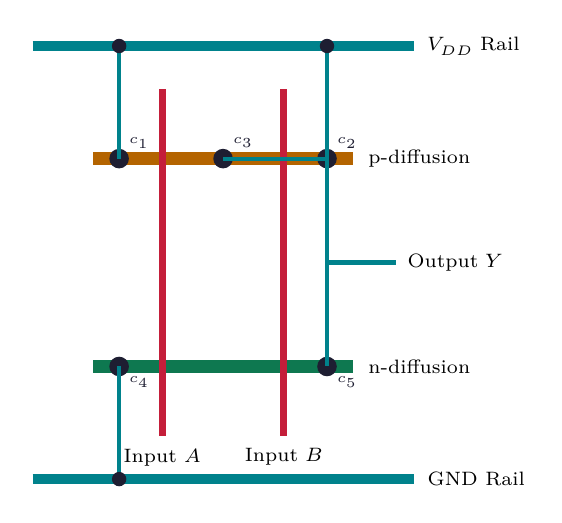
\begin{tikzpicture}[scale=1.1, thick, font=\small]
  % Rails (Metal 1 - Blue/Teal)
  \draw[draw=myteal, line width=3.5pt] (-2.2, 2.5) -- (2.2, 2.5) node[right, font=\scriptsize] {$V_{DD}$ Rail};
  \draw[draw=myteal, line width=3.5pt] (-2.2, -2.5) -- (2.2, -2.5) node[right, font=\scriptsize] {GND Rail};

  % Active Areas
  % p-Diffusion (Amber) - Horizontal
  \draw[draw=myamber, line width=4.5pt] (-1.5, 1.2) -- (1.5, 1.2) node[right, font=\scriptsize] {p-diffusion};
  % n-Diffusion (Green) - Horizontal
  \draw[draw=mygreen, line width=4.5pt] (-1.5, -1.2) -- (1.5, -1.2) node[right, font=\scriptsize] {n-diffusion};

  % Polysilicon Gates (Red) - Vertical
  \draw[draw=myred, line width=2.5pt] (-0.7, 2.0) -- (-0.7, -2.0) node[below, font=\scriptsize] {Input $A$};
  \draw[draw=myred, line width=2.5pt] (0.7, 2.0) -- (0.7, -2.0) node[below, font=\scriptsize] {Input $B$};

  % Contacts (Black circles) \& Connections (Teal lines)
  % p-diffusion contacts
  \filldraw[mydark] (-1.2, 1.2) circle (0.1) node[above right, font=\tiny] {$c_1$};
  \filldraw[mydark] (1.2, 1.2) circle (0.1) node[above right, font=\tiny] {$c_2$};
  \filldraw[mydark] (0, 1.2) circle (0.1) node[above right, font=\tiny] {$c_3$};

  % n-diffusion contacts
  \filldraw[mydark] (-1.2, -1.2) circle (0.1) node[below right, font=\tiny] {$c_4$};
  \filldraw[mydark] (1.2, -1.2) circle (0.1) node[below right, font=\tiny] {$c_5$};

  % VDD connections to pMOS sources
  \draw[draw=myteal, line width=1.5pt] (-1.2, 2.5) -- (-1.2, 1.2);
  \filldraw[mydark] (-1.2, 2.5) circle (0.07);
  \draw[draw=myteal, line width=1.5pt] (1.2, 2.5) -- (1.2, 1.2);
  \filldraw[mydark] (1.2, 2.5) circle (0.07);

  % GND connection to nMOS source (left side)
  \draw[draw=myteal, line width=1.5pt] (-1.2, -2.5) -- (-1.2, -1.2);
  \filldraw[mydark] (-1.2, -2.5) circle (0.07);

  % Output Connection (Metal 1)
  % Connect pMOS drain (center contact c3) and nMOS drain (right contact c5)
  \draw[draw=myteal, line width=1.5pt] (0, 1.2) -- (1.2, 1.2) -- (1.2, -1.2);
  \draw[draw=myteal, line width=1.5pt] (1.2, 0) -- (2.0, 0) node[right, font=\scriptsize] {Output $Y$};
\end{tikzpicture}
\end{tcolorbox}

\subsection{Lambda (\texorpdfstring{$\lambda$}{lambda}) vs. Micron Layout Rules}
Layout rules prevent defects like short-circuits or open circuits during manufacturing.
\begin{itemize}[leftmargin=*, itemsep=3.5pt]
  \item \textbf{Lambda-based rules (Mead-Conway):} Characterize the layout dimensions in terms of a scalable parameter $\lambda$, where $2\lambda$ equals the minimum feature size (channel length). Scaling the circuit to a new process node requires only updating the value of $\lambda$.
  \item \textbf{Micron-based rules:} Hard-coded absolute dimensions in micrometers/nanometers. Do not scale easily, requiring a complete redesign of the layout for a new technology, but yield tighter, more optimized layouts.
\end{itemize}

% ===============================================================================
\section{Physical Design Automation}
% ===============================================================================

Physical design automation translates a netlist into physical geometry on silicon through automated EDA tools.

\begin{enumerate}[label=\arabic*., leftmargin=*]
  \item \textbf{Partitioning:}
    \begin{itemize}
      \item \textbf{Goal:} Decompose a complex system containing millions of gates into smaller, manageable sub-chips or functional blocks.
      \item \textbf{Objective:} Minimize the number of cut nets (connections) crossing between different partitions to reduce routing congestion and delay.
    \end{itemize}
  \item \textbf{Floorplanning:}
    \begin{itemize}
      \item \textbf{Goal:} Plan the physical structure and block placement of the chip.
      \item \textbf{Objective:} Determine the shape, size, and approximate location of functional blocks (cores, RAMs). Establish the power distribution network (PDN grids) and pad structures. Optimize the chip aspect ratio and minimize dead area.
    \end{itemize}
  \item \textbf{Placement:}
    \begin{itemize}
      \item \textbf{Goal:} Assign exact physical coordinate locations to all standard cells within the floorplanned rows.
      \item \textbf{Objective:} Minimize total wire length, satisfy timing constraints, and avoid cell overlaps.
    \end{itemize}
  \item \textbf{Global Routing:}
    \begin{itemize}
      \item \textbf{Goal:} Plan the general paths for all signal wires across routing channels.
      \item \textbf{Objective:} Determine which channels or regions a net will traverse, optimizing congestion across the chip without defining the specific tracks yet. This is followed by \textbf{Detailed Routing}, which assigns wires to specific metal tracks and layers.
    \end{itemize}
\end{enumerate}

\newpage
% ===============================================================================
% MANDATORY QUICK REVISION PAGE
% ===============================================================================
\begin{center}
  {\large\bfseries\color{myred} Quick Revision --- Module 6}\\[3pt]
  {\small\color{mydark} Sizing, Power, Layout \& Physical Design Automation $|$ PE-EC603C}
\end{center}
\noindent{\color{myred}\rule{\linewidth}{1.2pt}}
\vspace{4pt}

\begin{tcolorbox}[formulabox, title={\textbf{Key Equations}}]
$$\text{Optimal Inverter Chain Sizing:} \quad f = e \approx 2.718 \qquad \text{Optimal Stages:} \quad N = \ln\left(\frac{C_L}{C_{in}}\right)$$
$$\text{Dynamic Power Dissipation:} \quad P_{dynamic} = \alpha C_L V_{DD}^2 f$$
$$\text{Static Power Dissipation:} \quad P_{static} = I_{leak} V_{DD} \qquad P_{total} = P_{dyn} + P_{sc} + P_{static}$$
$$\text{Lambda scale relationship:} \quad \text{Minimum Channel Length} = 2\lambda \qquad \text{Poly-to-Poly spacing} = 3\lambda$$
\end{tcolorbox}

\begin{tcolorbox}[defbox, title={\textbf{One-Line Definitions}}]
\begin{itemize}[leftmargin=*, itemsep=2.5pt, topsep=0pt]
  \item \textbf{Inverter Chain:} A cascade of progressively larger inverters designed to drive large capacitive loads with minimal delay.
  \item \textbf{Dynamic Power:} Power consumed by charging and discharging nodal capacitances during logical transitions.
  \item \textbf{Subthreshold Leakage:} Drain-source conduction current that flows when the gate-source voltage is below the threshold voltage.
  \item \textbf{Latch-Up:} A parasitic SCR trigger state creating a low-impedance short-circuit between supply rails, risking thermal failure.
  \item \textbf{Stick Diagram:} A cartoon layout representation using color-coded lines to show transistor connectivity.
  \item \textbf{Lambda ($\lambda$) Design Rules:} Mead-Conway layout rules parameterized by a scaling factor $\lambda$ to support easy node migration.
  \item \textbf{Floorplanning:} The EDA step determining shapes, sizes, and layout placements of block areas and power nets on a chip.
\end{itemize}
\end{tcolorbox}

\begin{tcolorbox}[exambox, title={\textbf{Frequently Asked / Viva Questions}}]
\begin{enumerate}[topsep=0pt, label=\textbf{Q\arabic*.}, itemsep=5pt]
  \item \Q{Derive the optimal scaling factor $f = e$ for an inverter chain.}
    The total delay of $N$ stages is $t_{path} = N f \tau_0$. Since $f^N = F \implies N = \ln(F)/\ln(f)$, substituting $N$ yields $t_{path} = \frac{\ln(F)}{\ln(f)} f \tau_0 = \ln(F) \tau_0 \frac{f}{\ln(f)}$. To minimize, differentiate with respect to $f$: $\frac{d}{d f}\left(\frac{f}{\ln(f)}\right) = \frac{\ln(f) - 1}{(\ln(f))^2} = 0 \implies \ln(f) = 1 \implies f = e$.
  \item \Q{Why does charging a capacitor from $V_{DD}$ dissipate energy in the pull-up network?}
    When charging a load capacitor $C_L$ to $V_{DD}$, the charge delivered is $Q = C_L V_{DD}$, drawing an energy of $E_{supply} = Q V_{DD} = C_L V_{DD}^2$. The final energy stored in the capacitor is $E_{cap} = \frac{1}{2} C_L V_{DD}^2$. By energy conservation, the remaining half of the energy is dissipated across the resistance of the conducting pMOS transistor as heat.
  \item \Q{Explain how subthreshold leakage current behaves in sub-micron technologies.}
    Subthreshold leakage is the current that flows between source and drain when $V_{GS} < V_{th}$. It is governed by diffusion and scales exponentially with lower threshold voltages ($I_{sub} \propto e^{(V_{GS}-V_{th})/n V_T}$). Thus, as technology scales and $V_{th}$ drops, static subthreshold power increases significantly.
  \item \Q{What is Latch-Up and how does it happen in CMOS?}
    CMOS structures contain parasitic PNP (p+ S/D, n-well, p-sub) and NPN (n+ S/D, p-sub, n-well) transistors forming a thyristor circuit. If noise injects current, it turns on one transistor, which then turns on the other, creating a self-sustaining low-impedance feedback path from $V_{DD}$ to GND that can burn out the chip.
  \item \Q{Explain the role of guard rings in preventing Latch-Up.}
    Guard rings are heavily doped $n^+$ regions in n-wells connected to $V_{DD}$ and $p^+$ regions in p-substrates connected to GND. They shunt stray currents by providing a low-resistance path to collect minority carriers, preventing the parasitic BJTs from turning ON.
  \item \Q{Describe the color coding standard used in Stick Diagrams.}
    Stick diagrams use: Blue for Metal 1 (routing and rails), Red for Polysilicon (gate contacts), Green for n-diffusion (nMOS active channel), Amber/Yellow for p-diffusion (pMOS active channel), and black dots/crosses for layer connection contacts.
  \item \Q{Compare Lambda-based and Micron-based design rules.}
    Lambda-based design rules scale layout shapes by a parameter $\lambda$ (equal to half the minimum feature size), making migration to new technology nodes automatic by changing $\lambda$. Micron-based design rules use absolute physical dimensions, which are harder to scale but yield much denser layouts.
  \item \Q{What are the primary objectives of partitioning in physical design?}
    Partitioning divides a large netlist into smaller sub-blocks. Its primary objective is to minimize the number of interconnect wires crossing the boundaries of partitions, which reduces routing congestion, propagation delay, and improves overall layout efficiency.
  \item \Q{Explain the difference between Global Routing and Detailed Routing.}
    Global Routing plans the rough paths of all signal nets, deciding which channels or routing regions they will pass through to balance routing congestion. Detailed Routing takes this plan and assigns the nets to specific metal tracks and layers, complying with spacing and design rules.
  \item \Q{Why is floorplanning crucial for high-performance VLSI chips?}
    Floorplanning determines the physical locations and dimensions of functional blocks and coordinates the power supply network. It is crucial because early decisions on block placement set bounds on the length of global interconnect wires, which dominate routing delays and power consumption.
\end{enumerate}
\end{tcolorbox}

\begin{tcolorbox}[tikzbox, title={Lambda ($\lambda$) rules vs. Micron rules}]
\renewcommand{\arraystretch}{1.4}
\par\noindent
\begin{tabularx}{\linewidth}{|B{3.2cm}|Y|Y|}
\hline
\textbf{Feature} & \textbf{\color{myred}Lambda-based ($\lambda$) Rules} & \textbf{\color{myteal}Micron-based Rules} \\
\hline
\textbf{Scaling} & Highly scalable (dimensions scaled by $\lambda$). & Not scalable (absolute physical dimensions). \\
\hline
\textbf{Density} & Sub-optimal (oversized clearances). & Highly optimized (maximum density). \\
\hline
\textbf{Complexity} & Simple and easy to learn. & Complex, process-specific specifications. \\
\hline
\textbf{Migration} & Auto-migration to new fabrication nodes. & Requires manual redesign of layout. \\
\hline
\textbf{Application} & Academic designs and prototyping. & Industry-standard product tape-outs. \\
\hline
\end{tabularx}
\tcbset{colbacktitle=mypurple, coltitle=white}
\end{tcolorbox}

\end{document}
